%==============================================================================
%  Smart City Surveillance System - Digital Image Processing
%
%  IEEE conference format (double column). Compiles on Overleaf with
%  pdfLaTeX -> BibTeX -> pdfLaTeX -> pdfLaTeX.
%==============================================================================
\documentclass[conference,10pt]{IEEEtran}

\usepackage[T1]{fontenc}
\usepackage[utf8]{inputenc}
\usepackage{graphicx}
\usepackage{amsmath}
\usepackage{amssymb}
\usepackage{booktabs}
\usepackage{array}
\usepackage{multirow}
\usepackage{balance}
\usepackage[hidelinks]{hyperref}
\usepackage{url}

% IEEEtran's conference mode locks out \thanks; re-enable it so the
% repository link can sit in a footnote instead of the title block
\IEEEoverridecommandlockouts

\graphicspath{{figures/}}

% tighter float packing - keeps a float-heavy paper from spilling pages
\renewcommand{\topfraction}{0.95}
\renewcommand{\bottomfraction}{0.95}
\renewcommand{\textfraction}{0.05}
\renewcommand{\floatpagefraction}{0.85}
\setlength{\textfloatsep}{7pt plus 2pt minus 2pt}
\setlength{\floatsep}{7pt plus 2pt minus 2pt}
\setlength{\intextsep}{7pt plus 2pt minus 2pt}

% compact table typography used throughout
\newcommand{\hdr}[1]{\textbf{#1}}
\newcolumntype{R}{>{\raggedleft\arraybackslash}X}

\begin{document}

\title{An Adaptive Digital Image Processing Pipeline for\\
Smart-City Surveillance under Noise, Low Light,\\
Interference and Transmission Loss}

\author{%
\IEEEauthorblockN{Muhammad Abdullah Akram}
\IEEEauthorblockA{F2022065063}
\and
\IEEEauthorblockN{Gulshan Aslam}
\IEEEauthorblockA{F2022065206}
\and
\IEEEauthorblockN{Laiba Saeed}
\IEEEauthorblockA{F2022065207}
\and
\IEEEauthorblockN{Jawad Ahmad}
\IEEEauthorblockA{F2022065111}
\thanks{Code and data: \url{https://github.com/U-LF/smart-surveillance-dip}}}

\maketitle

%==============================================================================
\begin{abstract}
%==============================================================================
Islamabad's public-space surveillance network suffers from sensor noise,
under-exposed night frames, electrical interference, motion blur and packet
loss, all of which degrade the identification of pedestrians and vehicles. We
present a complete image-processing pipeline that treats these faults as an
inverse problem rather than a fixed filter chain: five blind diagnostics
measure each frame, and only the restoration stages the diagnosis actually
calls for are executed, with a user-selected \emph{profile} capping how
expensive each stage may be. The system implements six technical tasks---spatial filtering, frequency-domain filtering, restoration
and reconstruction, edge- and region-based segmentation, JPEG and wavelet
compression, and object recognition---with the core operators written from
first principles and verified against reference libraries. Every design
trade-off is measured rather than asserted. Blind diagnosis flags Gaussian
noise, impulse noise, periodic interference, night exposure and packet loss in
100\,\% of degraded frames at a false-alarm rate of at most 5\,\% on clean
frames. Adaptive restoration raises pedestrian $F_1$ from 0.624 to 0.917 under
20\,\% salt-and-pepper noise and from 0.509 to 0.733 on compound night frames.
Marker-controlled watershed segmentation attains IoU 0.692 at 3.5\,ms per
frame, beating GrabCut on both accuracy and cost. Region-of-interest coding
gains 7.0\,dB on people at equal file size in a wide CCTV view, and pixelating
heads preserves analytics ($F_1$ 0.877 versus 0.900) while removing identities.
Evaluation on real CCTV shows detection is limited by object scale rather than
image quality. The profiles span real-time and quality regimes on one CPU with
no GPU.
\end{abstract}

\begin{IEEEkeywords}
Digital image processing, video surveillance, image restoration, image
segmentation, image compression, object detection, privacy protection,
real-time systems.
\end{IEEEkeywords}

%==============================================================================
\section{Introduction}\label{sec:intro}
%==============================================================================
\IEEEPARstart{T}{he} city of Islamabad has deployed a smart surveillance system
for real-time monitoring of public spaces. In practice the deployment is
limited less by the analytics than by the quality of the imagery reaching them:
cameras operate at night with short exposure and high sensor gain, share
infrastructure with power electronics that inject periodic interference,
observe fast-moving vehicles that motion-blur, and stream over wireless links
that drop packets. The result is that pedestrians and vehicles which a detector
would find easily in clean imagery are missed.

A conventional response is a fixed enhancement chain---denoise, sharpen,
brighten---applied to every frame. This is wasteful, because a clean daytime
frame pays for filters it does not need on a node whose compute budget is
shared across many cameras; and harmful, because enhancement operators are not
benign: a median filter erases fine detail, non-local means removes the weak
edges edge-based segmentation depends on, and histogram equalisation amplifies
exactly the noise a dark frame contains most of.

This work therefore treats frame enhancement as a \emph{decision} problem. The
system measures the frame---noise standard deviation, impulse density, spectral
peak prominence, mean luminance, dark-region fraction and lost-block
ratio---then executes only the operators those measurements justify. A profile
(\textsf{fast}, \textsf{balanced}, \textsf{quality}) independently caps the cost
of each selected operator, converting the real-time-versus-quality requirement
from a discussion point into a run-time parameter.

\subsection{Contributions}
\begin{enumerate}
\item A \emph{blind diagnostic front end} calibrated against measured
      false-alarm rates on clean imagery, establishing which faults are
      separable from frame statistics alone---and which are not.
\item An \emph{adaptive restoration pipeline} whose stage ordering is
      justified experimentally rather than by convention, including two
      non-obvious orderings: repairing pixel-level defects before any
      resampling, and judging noise by its post-brightening magnitude.
\item \emph{From-scratch implementations} of the core operators---convolution,
      median and adaptive median filters, the DFT filter family, Otsu,
      histogram equalisation, region growing, an 8$\times$8 DCT codec and a
      wavelet codec---each verified against OpenCV or scikit-image.
\item A \emph{measured account of every design trade-off}, with
      the negative results retained: uneven illumination is not blindly
      detectable, denoising before segmentation does not help, and the largest
      detector input size is not the most accurate.
\item An explicit \emph{module interdependence} analysis quantifying what each
      upstream stage is worth to the downstream task.
\end{enumerate}

%==============================================================================
\section{Problem Analysis and Constraints}\label{sec:problem}
%==============================================================================

\subsection{Fault taxonomy and the degradation model}
Public surveillance datasets contain reasonably clean imagery, whereas
PSNR and SSIM require a known clean reference that real night footage cannot
provide. We therefore adopt the standard linear degradation model
\cite{gonzalez2018}
\begin{equation}
g(x,y) \;=\; H\!\left[f(x,y)\right] \;+\; \eta(x,y),
\label{eq:degradation}
\end{equation}
where $f$ is the clean frame, $H$ a (possibly identity) degradation operator
and $\eta$ an additive noise field, and synthesise each fault with documented,
seeded parameters. Seven faults are modelled: Gaussian sensor noise, salt-and-pepper
bit errors, sinusoidal mains interference, linear motion blur, under-exposure,
a multiplicative illumination field, and zeroed 16$\times$16 blocks standing
for dropped packets. A compound ``worst night'' scenario combines
under-exposure, sensor noise and sparse bit errors, because real failures
co-occur.

\subsection{Constraints}
Three constraints shape every design decision that follows.

\textit{Real-time performance versus processing quality.} A node must keep up
with its camera. Restoration cost is dominated by a few expensive operators
(non-local means, per-frame FFT, large detector inputs), so the system must be
able to trade them away rather than being compiled around one fixed choice.

\textit{Resource constraints versus performance.} The target is an edge-class
device without a GPU, which rules out large detectors, motivates YOLOv4-tiny
through OpenCV's DNN module (no PyTorch, no CUDA), and makes peak memory a
reported metric.

\textit{Security and privacy versus system accessibility.} A stream that
exposes identities is a liability, but one that destroys them also destroys the
analytics justifying the system. The design must hide identity while preserving
the evidence counting and tracking depend on, and let an authorised
investigator recover the original.

%==============================================================================
\section{System Design: Pipeline and Flowcharts}\label{sec:design}
%==============================================================================

\begin{figure*}[!t]
\centering
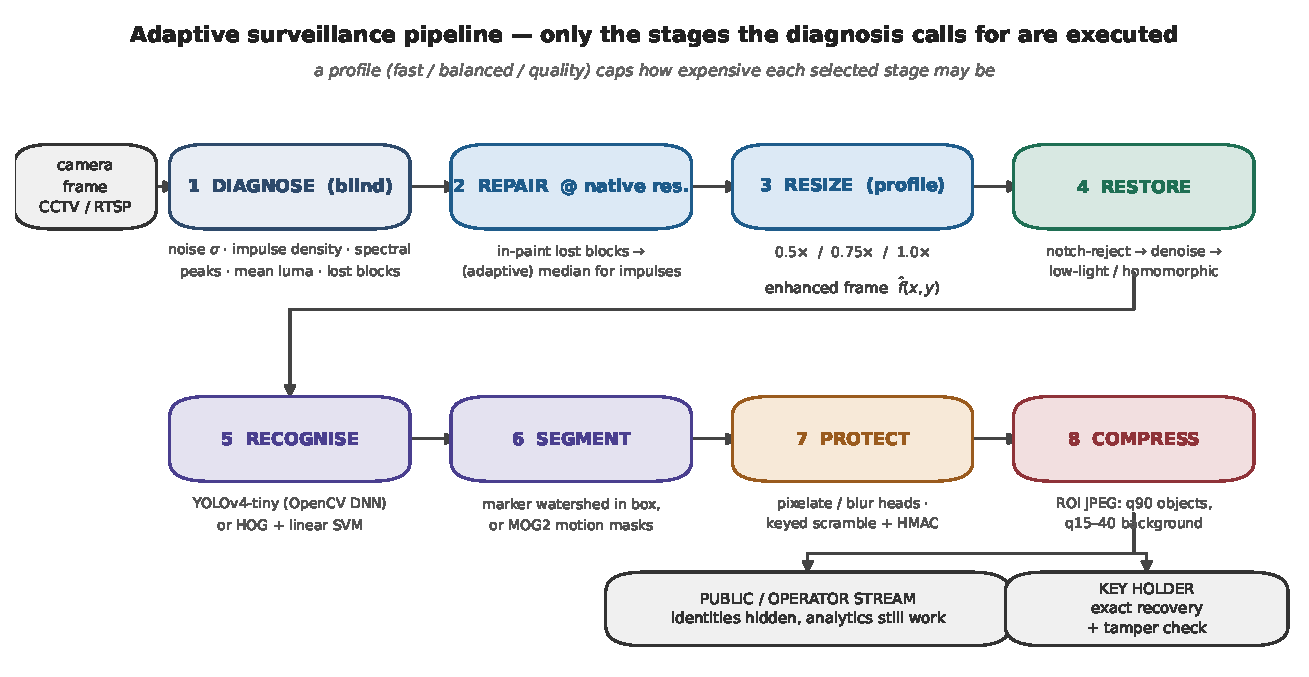
\includegraphics[width=0.82\textwidth]{fig_pipeline.pdf}
\caption{End-to-end system pipeline. Stages 1--2 run at native resolution
because area resampling would average impulses and lost blocks into blobs that
no later filter can identify; the profile then fixes the working resolution and
the cost ceiling of every subsequent stage. Detection boxes are the common
currency of stages 6--8: they tell segmentation \emph{where} to look, privacy
\emph{what} to hide and the codec \emph{which} regions deserve bits.}
\label{fig:pipeline}
\end{figure*}

\subsection{Pipeline overview}
Fig.~\ref{fig:pipeline} shows the eight stages: the frame is diagnosed and
pixel-level defects repaired at native resolution; the profile rescales it;
restoration removes interference, noise and lighting defects; a detector
locates people and vehicles; segmentation refines those boxes into
silhouettes; a privacy stage hides identities; and a region-of-interest codec
spends bits where the objects are. Only the selected stages execute.

\subsection{Adaptive decision logic}
Fig.~\ref{fig:flowchart} is the decision flowchart actually implemented in
\texttt{surveillance/pipeline.py}; the thresholds printed on it are read from
the source at drawing time, so the figure cannot drift from the code.
Table~\ref{tab:thresholds} lists each threshold together with the measured
separation that justifies it.

\begin{figure}[!t]
\centering
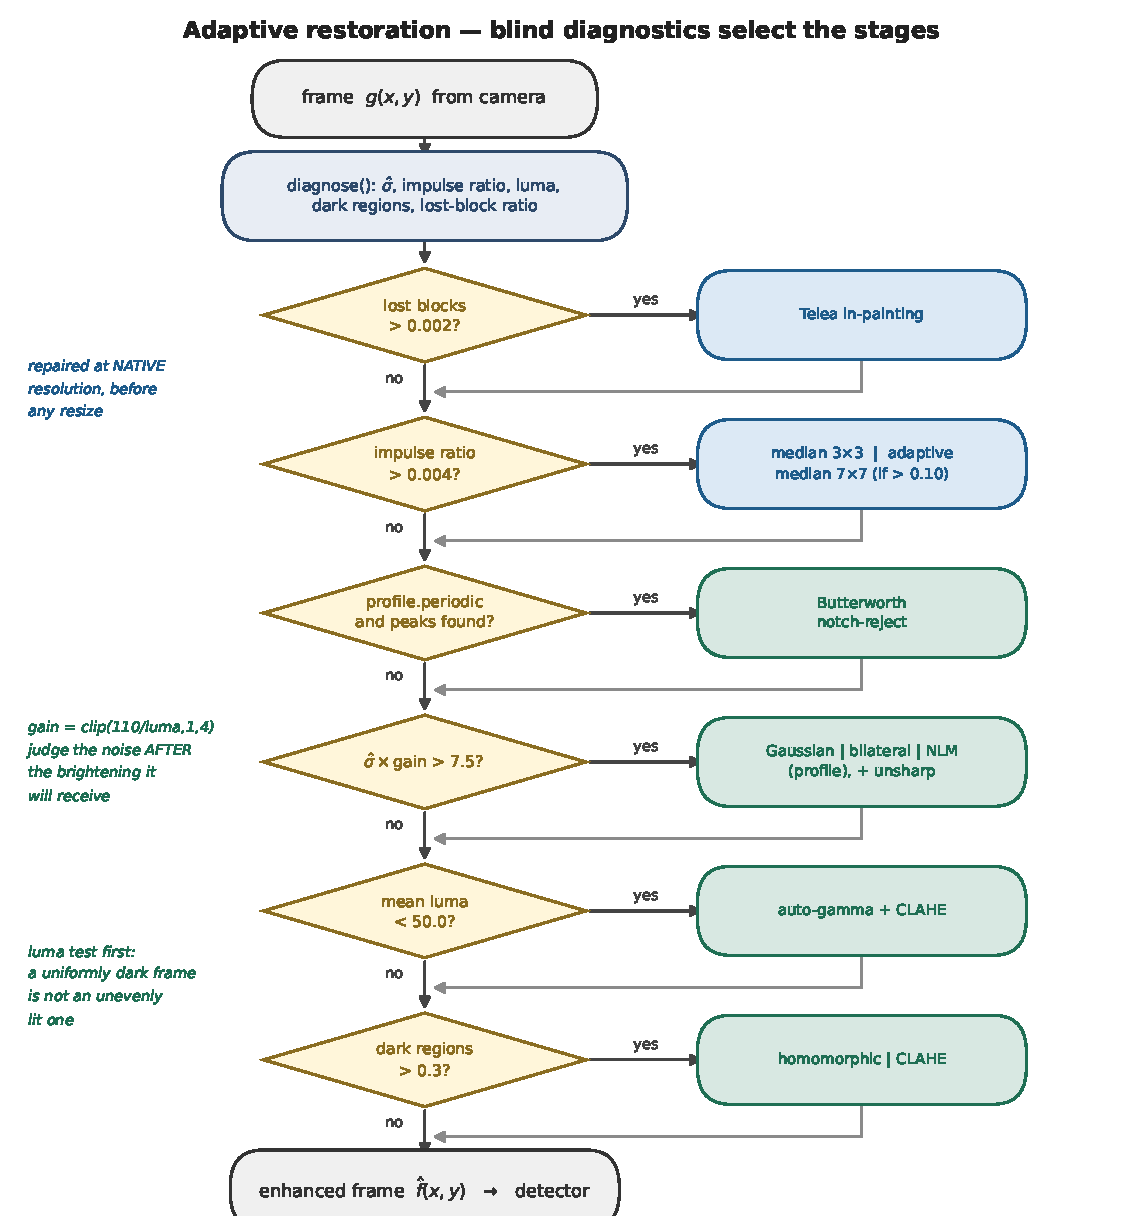
\includegraphics[width=0.74\columnwidth]{fig_flowchart.pdf}
\caption{Adaptive restoration flowchart. Each diamond is a blind test on the
diagnostics; the ``yes'' branch executes an operator whose strength is set by
the profile, and control rejoins the main path. Three orderings are
deliberate and are justified in Section~\ref{sec:design-order}.}
\label{fig:flowchart}
\end{figure}

\begin{table}[!t]
\caption{Decision thresholds and the measured separation justifying each
(Section~\ref{sec:res-diag}).}
\label{tab:thresholds}
\centering
\scriptsize
\begin{tabular}{@{}lrp{3.5cm}@{}}
\toprule
\hdr{Statistic} & \hdr{Threshold} & \hdr{Measured separation} \\
\midrule
impulse ratio      & $0.004$ & clean $\le 0.001$; 5\,\% S\&P $\ge 0.033$ \\
noise $\hat\sigma$ & $7.5$   & clean 0.6--8.1 (95th pct.\ 5.8); $\sigma{=}15 \Rightarrow \ge 9.4$ \\
mean luminance     & $50$    & clean $\ge 62$; simulated night 12--34 \\
dark-region frac.  & $0.30$  & \emph{not} separable --- see Section~\ref{sec:limits} \\
lost-block ratio   & $0.002$ & clean $0$; 3\,\% loss $\approx 0.028$ \\
spectral prominence& $2.0$   & clean $<2.0$; amplitude-40 interference 1.6--4.3 \\
\bottomrule
\end{tabular}
\end{table}

\subsection{Profiles}
A profile is one object fixing the working resolution and the cost ceiling of
each stage (Table~\ref{tab:profiles}). It never changes \emph{whether} an
operator runs---that remains the diagnosis's decision---only \emph{how
expensive} it may be.

\begin{table}[!t]
\caption{The three operating profiles.}
\label{tab:profiles}
\centering
\scriptsize
\begin{tabular}{@{}lccc@{}}
\toprule
 & \hdr{fast} & \hdr{balanced} & \hdr{quality} \\
\midrule
resolution        & $0.5\times$   & $0.75\times$  & $1.0\times$ \\
impulse filter    & median 3$\times$3 & median 3$\times$3 & adaptive median \\
denoiser          & Gaussian      & bilateral     & NLM + unsharp \\
periodic notch    & --            & yes           & yes \\
illumination      & gamma         & gamma+CLAHE   & \,+\,homomorphic \\
detector input    & 320, every 3rd & 416          & 608 \\
segmentation      & MOG2 masks    & watershed     & watershed \\
JPEG $q$ (ROI/bg) & 85 / 25       & 90 / 30       & 92 / 40 \\
\bottomrule
\end{tabular}
\end{table}

\subsection{Three deliberate orderings}\label{sec:design-order}
\textit{(i) Repair before resize.} Area-interpolated downsampling averages an
isolated saturated pixel into its neighbourhood, converting a detectable
impulse into an undetectable local bias; the same applies to a zeroed
16$\times$16 block. Both are therefore repaired at native resolution.

\textit{(ii) Denoise before brightening, judged after gain.} Low-light
enhancement multiplies intensities by an effective gain
$\gamma \approx \mathrm{clip}(110/\bar{L},\,1,\,4)$, so noise invisible in a
dark frame is amplified into visibility. The system tests
$\hat\sigma\cdot\gamma$ rather than $\hat\sigma$, and denoises \emph{before}
enhancing.

\textit{(iii) Luminance before uniformity.} A uniformly dark frame and an
unevenly lit one need opposite corrections, so only a frame bright \emph{on
average} is considered for homomorphic correction.

\textit{(iv) Re-estimate after repair.} Noise is re-estimated after impulse and
notch removal, since both change the residual the denoiser must match.

%==============================================================================
\section{Methods}\label{sec:methods}
%==============================================================================
This section maps the six technical tasks onto the implementation.
Operators marked \emph{(scratch)} are written from first principles and
verified in Section~\ref{sec:setup}.

\subsection{Task 1: Spatial filtering}
Two-dimensional correlation \emph{(scratch)} with reflect-101 borders
underpins the mean and Laplacian filters, and the median is implemented
\emph{(scratch)} with sliding-window order statistics. The \emph{adaptive
median} \cite{gonzalez2018} grows its window until the local median is not
itself an impulse ($z_{\min} < z_{\mathrm{med}} < z_{\max}$) and replaces a
pixel only when that pixel is extreme, preserving detail where a fixed median
smears it. Edge-preserving smoothing uses the bilateral filter
\cite{tomasi1998bilateral} with $\sigma_{\mathrm{color}}$ tied to the estimated
noise, and non-local means \cite{buades2005nlm} in the quality profile.

\subsection{Task 2: Frequency-domain filtering}
The ideal, Butterworth and Gaussian low- and high-pass transfer functions
$H(u,v)$ are built on a centred distance grid and applied as
$g=\mathcal{F}^{-1}\{H\cdot\mathcal{F}\{f\}\}$ with reflect padding, with
cut-offs expressed as a fraction of image size for resolution independence.

The interference remover is automatic: the Hann-windowed log-magnitude spectrum
is scored for spikes by subtracting, at each frequency, the mean of an annulus
$4 \le r \le 9$ bins away from the mean of the $3\times3$ core---a pure
sinusoid concentrates into the core while the $1/f$ scene background is flat
across both---and conjugate-symmetric peaks above a prominence of 2.0 are
suppressed with an order-4 Butterworth notch-reject product filter. Uneven
lighting is handled homomorphically: since $f = i\cdot r$, logarithms separate
illumination from reflectance, so attenuating low frequencies
($\gamma_L{=}0.4$) while preserving high ones ($\gamma_H{=}1.1$) flattens the
illumination field without flattening the scene.

\subsection{Task 3: Restoration and reconstruction}
Deconvolution is implemented as the inverse filter $\hat{F}=G/H$, the Wiener
filter $\hat{F} = \left[H^{*}/(|H|^{2}+K)\right]G$, and constrained least
squares with a Laplacian penalty. Low-light restoration offers auto-gamma,
global histogram equalisation \emph{(scratch)} and CLAHE
\cite{zuiderveld1994clahe}; lost blocks are located by an all-black block test
and filled by Telea in-painting \cite{telea2004}.

Blind diagnostics use an edge-aware Immerk{\ae}r estimator
\cite{immerkaer1996}: the difference-of-Laplacians response is summed only over
the 70\,\% of pixels with the weakest Sobel response \cite{tai2008}, because
the plain estimator over-reads on textured streets.

\subsection{Task 4: Segmentation}
Both families are implemented and compared inside detector boxes, which is how
a surveillance system uses segmentation: the detector says \emph{where}, the
segmenter says \emph{which pixels}. Edge-based methods use Canny
\cite{canny1986} or Sobel gradients followed by morphological closing, hole
filling and largest-component selection. Region-based methods are Otsu
\emph{(scratch)} \cite{otsu1979} on a colour-distance map, seeded region
growing \emph{(scratch)}, marker-controlled watershed and
GrabCut \cite{rother2004}. For static cameras a motion segmenter combines MOG2
\cite{zivkovic2004}---or a from-scratch running average---with morphology and
connected components.

\subsection{Task 5: Compression}
Baseline JPEG through libjpeg is the production reference. A
from-scratch JPEG-like codec performs colour transform, 4:2:0 subsampling,
8$\times$8 DCT, IJG-scaled quantisation, zig-zag scan, DC differential coding
and entropy coding, exposing every stage; a wavelet codec
\cite{antonini1992} applies a multi-level DWT with dead-zone
quantisation. All three report \emph{measured} compressed byte counts, so bits
per pixel is observed rather than estimated. Region-of-interest coding encodes
detected objects at high quality and the background at low quality, resolving
the compression--fidelity trade-off per region instead of per frame.

\subsection{Task 6: Object recognition}
Two detectors share one interface: HOG with a linear SVM \cite{dalal2005} as
the classical baseline, and YOLOv4-tiny \cite{bochkovskiy2020} through
OpenCV's DNN module, detecting people and vehicles at three input sizes on a
CPU. Greedy non-maximum suppression is implemented \emph{(scratch)}.

\subsection{Privacy and evidence integrity}
Three tiers are provided \cite{ribaric2016privacy}: irreversible anonymisation
(pixelating or blurring heads, bodies or silhouettes) for the public stream; a
keyed scrambler permuting 8$\times$8 blocks under a key-derived keystream, from
which a key holder recovers the original bit-exactly; and an HMAC-SHA256 tag
\cite{nist2008hmac} per stored frame so tampering is detectable.

%==============================================================================
\section{Experimental Setup}\label{sec:setup}
%==============================================================================

\subsection{Datasets}
Table~\ref{tab:data} lists the data used. Penn-Fudan \cite{wang2007pennfudan} is the primary still-image set because it
is the only freely available pedestrian set with \emph{pixel-accurate instance
masks}, which IoU and Dice require and bounding-box datasets cannot supply; its
clean frames also serve as the references \eqref{eq:degradation} demands.
CAVIAR \cite{caviar2004} supplies real CCTV with hand-labelled boxes and a
KITTI \cite{geiger2012kitti} clip supplies vehicles.

Three candidate datasets are deliberately not used. Cityscapes
\cite{cordts2016cityscapes} requires registered access and roughly 12\,GB,
conflicting with the requirement that every result be regenerable from one
unattended download. The Lahore Urban Traffic Observations set is tabular
sensor data, not imagery. A face-mask dataset addresses mask classification on
tightly cropped faces---orthogonal to the six tasks, and exercising neither
restoration nor compression under realistic surveillance geometry.

\begin{table}[!t]
\caption{Data used. All sources download without registration and are verified
on arrival (file counts, MD5, XML parse).}
\label{tab:data}
\centering
\scriptsize
\begin{tabular}{@{}p{1.7cm}p{2.1cm}p{3.3cm}@{}}
\toprule
\hdr{Dataset} & \hdr{Content} & \hdr{Used for} \\
\midrule
Penn-Fudan \cite{wang2007pennfudan} & 170 images, 423 mask instances & PSNR/SSIM references, IoU/Dice, $P$/$R$/$F_1$ \\
CAVIAR \cite{caviar2004} & 5 sequences, 2211 frames, CVML boxes & real-CCTV detection, motion segmentation \\
KITTI clip \cite{geiger2012kitti} & 16.6\,s street video & vehicle robustness \\
\texttt{vtest.avi} & 768$\times$576, static camera & real-time benchmark, ROI coding \\
YOLOv4-tiny \cite{bochkovskiy2020} & COCO weights, 24\,MB & recognition \\
\bottomrule
\end{tabular}
\end{table}

\subsection{Metrics}
Image quality uses MSE, PSNR and SSIM \cite{wang2004ssim}; segmentation uses
IoU and Dice; detection uses greedy score-ordered one-to-one matching at
IoU~$0.5$ with precision, recall, $F_1$ and all-point interpolated AP
\cite{everingham2010voc}. Because Penn-Fudan leaves small and heavily occluded
people unlabelled, unmatched detections shorter than 90\,px are ignored rather
than counted as false positives, identically for every detector.

\subsection{Verification and reproducibility}
Every from-scratch operator is checked against an independent reference in a
17-test suite: convolution against \texttt{cv2.filter2D} to $10^{-8}$; mean and
median filters against OpenCV exactly; Otsu and histogram equalisation to
within one grey level; PSNR and SSIM against scikit-image; and the scrambler
against exact round-trip and key-sensitivity properties. All randomness is
seeded, so the result set regenerates from one command. Experiments ran
single-process on an Apple~M-series CPU with Python~3.14, OpenCV~4.14 and
NumPy~2.5.

%==============================================================================
\section{Results and Analysis}\label{sec:results}
%==============================================================================

\subsection{Can each fault be detected blindly?}\label{sec:res-diag}
Before any filter can be selected adaptively, the system must be able to
recognise what is wrong with a frame using only the frame itself.
Table~\ref{tab:trigger} is the resulting trigger matrix over 60 images: each
row is a scenario, each column the percentage of frames on which a given
diagnostic fired.

\begin{table}[!t]
\caption{Trigger matrix (\% of 60 frames on which each diagnostic fires).
Diagonal entries are correct detections; the \emph{clean} row is the
false-alarm rate.}
\label{tab:trigger}
\centering
\scriptsize
\begin{tabular}{@{}lrrrrrr@{}}
\toprule
\hdr{Scenario} & \hdr{imp.} & \hdr{noise} & \hdr{per.} & \hdr{dark} & \hdr{d.reg} & \hdr{lost} \\
\midrule
clean            & 0 & 2 & 5 & 0 & 0 & 0 \\
Gaussian $\sigma{=}15$ & 0 & \textbf{100} & 5 & 0 & 0 & 0 \\
Gaussian $\sigma{=}30$ & 0 & \textbf{100} & 5 & 0 & 0 & 0 \\
salt \& pepper 5\,\%   & \textbf{100} & 100 & 5 & 0 & 0 & 0 \\
salt \& pepper 20\,\%  & \textbf{100} & 100 & 0 & 0 & 0 & 0 \\
periodic         & 0 & 2 & \textbf{100} & 0 & 0 & 0 \\
motion blur      & 0 & 0 & 5 & 0 & 0 & 0 \\
low light        & 0 & 0 & 3 & \textbf{100} & 0 & 0 \\
uneven light     & 0 & 0 & 5 & 2 & \textit{5} & 2 \\
block loss       & 0 & 2 & 2 & 0 & 2 & \textbf{100} \\
night compound   & \textbf{100} & 53 & 5 & \textbf{100} & 0 & 0 \\
\bottomrule
\end{tabular}
\end{table}

Five of the six fault classes are detected on 100\,\% of degraded frames while
firing on at most 5\,\% of clean frames. The compound night scenario triggers
both the impulse and darkness rules; its noise rule fires on only 53\,\% of
frames, an under-detection the gain-aware test of
Section~\ref{sec:design-order} compensates, since a frame flagged as dark has
its noise re-evaluated after the brightening gain.


The noise estimator is monotonic in true $\sigma$ but systematically
under-reads it---10.7 at $\sigma{=}15$, 19.5 at $\sigma{=}30$, 25.0 at
$\sigma{=}40$---because clipping at 0 and 255 discards noise energy and the
homogeneous-region restriction samples the flattest 70\,\% of the image. This
is acceptable because the threshold was calibrated against the estimator's
measured output (clean frames average 2.4, maximum 8.7; $\sigma{=}15$ yields a
minimum of 9.8) rather than nominal $\sigma$: separation at the decision
boundary, not absolute accuracy, is what the pipeline requires.

Periodic interference detection rises with amplitude: 5\,\% at amplitude 0 (the
false-alarm floor, caused by periodic scene content such as railings), 81.7\,\%
at 10, 98.3\,\% at 20 and 100\,\% at 40 and above.

The one clear negative result is uneven illumination, whose diagnostic fires on
only 5\,\% of frames---indistinguishable from the clean false-alarm rate. A
clean street scene with ordinary shadows produces the same dark-region
statistic as genuinely non-uniform lighting, because the statistic cannot tell
a dark \emph{object} from a dark \emph{illuminant}. Rather than tune the
threshold until it appears to work, we report it as unusable and expose
homomorphic correction as a per-camera setting
(\texttt{illumination="always"}).

\subsection{Task 1: Spatial filtering}\label{sec:res-spatial}
Table~\ref{tab:spatial} reports the best filter per scenario together with the
cost of obtaining it, using the \emph{blind} $\hat\sigma$ estimate to set filter
strength, exactly as the deployed system would.

\begin{table}[!t]
\caption{Spatial filtering (40 images). Best filter per scenario, compared with
the cheapest competitive alternative.}
\label{tab:spatial}
\centering
\scriptsize
\begin{tabular}{@{}llrrr@{}}
\toprule
\hdr{Scenario} & \hdr{Filter} & \hdr{PSNR} & \hdr{SSIM} & \hdr{ms} \\
\midrule
\multirow{3}{*}{Gaussian $\sigma{=}15$}
 & (degraded)        & 24.77 & 0.591 & --- \\
 & \textbf{NLM}      & \textbf{28.51} & \textbf{0.795} & 208.6 \\
 & Gaussian          & 27.35 & 0.792 & \textbf{0.3} \\
\midrule
\multirow{3}{*}{Gaussian $\sigma{=}30$}
 & (degraded)        & 19.02 & 0.362 & --- \\
 & \textbf{Gaussian} & \textbf{24.47} & \textbf{0.676} & \textbf{0.4} \\
 & NLM               & 24.28 & 0.660 & 208.5 \\
\midrule
\multirow{4}{*}{S\&P 5\,\%}
 & (degraded)        & 17.93 & 0.448 & --- \\
 & \textbf{adaptive median} & \textbf{31.83} & \textbf{0.945} & 15.5 \\
 & median 3$\times$3 & 27.82 & 0.851 & \textbf{0.2} \\
 & bilateral         & 17.91 & 0.430 & 1.4 \\
\midrule
\multirow{3}{*}{S\&P 20\,\%}
 & (degraded)        & 11.92 & 0.153 & --- \\
 & \textbf{adaptive median} & \textbf{29.42} & \textbf{0.925} & 17.1 \\
 & median 3$\times$3 & 24.97 & 0.795 & \textbf{0.1} \\
\bottomrule
\end{tabular}
\end{table}

The \emph{matched} filter matters far more than the expensive one. On 20\,\%
impulse noise the adaptive median gains 17.5\,dB over the degraded input and
4.4\,dB over a fixed 3$\times$3 median, whereas non-local means---the most
expensive filter available, at 208\,ms---reaches only 16.34\,dB, some 13\,dB
worse, because an averaging filter cannot repair saturated outliers. Bilateral
filtering is worse still (12.12\,dB), since an impulse is precisely the large
intensity difference its range kernel is designed to preserve. Choosing the
wrong filter family costs far more than choosing a cheap member of the right
one---the entire justification for diagnosing before filtering.

The cost/benefit picture for Gaussian noise is equally pointed. At
$\sigma{=}15$ non-local means is best (28.51\,dB) but takes 208.6\,ms, while a
simple Gaussian blur reaches 27.35\,dB---96\,\% of the SSIM---in 0.3\,ms, a
$700\times$ speed-up for 1.2\,dB. At $\sigma{=}30$ the Gaussian filter
\emph{overtakes} NLM outright (24.47 versus 24.28\,dB). This is why the
\textsf{fast} profile's cheap Gaussian denoiser is not merely a compromise, and
why NLM is confined to the \textsf{quality} profile.

Sharpening after denoising is counter-productive in every scenario tested:
\texttt{median3+laplacian} and \texttt{nlm+unsharp} always score below the
corresponding filter alone, because both amplify the residual noise the
denoiser left behind. Sharpening is consequently gated behind the
\textsf{quality} profile and applied only at low amplitude.

\subsubsection{From-scratch implementations versus OpenCV}
The scratch NumPy implementations are numerically \emph{identical} to OpenCV's
(maximum absolute difference 0 for all four operators) while being
5--305$\times$ slower: mean 5$\times$5, 8.16 versus 0.07\,ms; median
3$\times$3, 19.89 versus 0.07\,ms ($305\times$); median 5$\times$5, 65.05
versus 0.23\,ms; Laplacian, 4.11 versus 0.79\,ms ($5.2\times$). The scratch
versions demonstrate the mechanism and validate the library; the library
versions serve the real-time path. The Laplacian's smaller gap reflects a
3$\times$3 kernel dominated by memory traffic rather than the arithmetic SIMD
accelerates in the median's sorting network.

\subsection{Task 2: Frequency-domain filtering}\label{sec:res-freq}
\subsubsection{Periodic interference}
Table~\ref{tab:periodic} compares the automatic notch-reject filter against
global low-pass filtering and spatial smoothing on frames corrupted with
randomly placed sinusoidal interference.

\begin{table}[!t]
\caption{Removing periodic interference (30 images, random interference
frequencies).}
\label{tab:periodic}
\centering
\scriptsize
\begin{tabular}{@{}lrrr@{}}
\toprule
\hdr{Method} & \hdr{PSNR} & \hdr{SSIM} & \hdr{ms} \\
\midrule
(degraded)                 & 22.30 & 0.530 & --- \\
spatial mean 5$\times$5    & 23.07 & 0.546 & 0.2 \\
spatial median 5$\times$5  & 23.22 & 0.539 & 0.3 \\
ideal LPF $D_0{=}0.10$     & 22.01 & 0.512 & 44.1 \\
Butterworth LPF $D_0{=}0.10$ & 23.12 & 0.594 & 49.9 \\
Gaussian LPF $D_0{=}0.10$  & 23.35 & 0.592 & 46.1 \\
\textbf{auto notch-reject} & \textbf{34.78} & \textbf{0.943} & 94.9 \\
\bottomrule
\end{tabular}
\end{table}

The notch filter gains \textbf{12.5\,dB} over the degraded input against at
most 1.1\,dB for the best global low-pass---an order-of-magnitude difference
that illustrates the central argument for frequency-domain processing. Periodic
interference is spatially delocalised but spectrally compact: it occupies two
conjugate points in $F(u,v)$ and everywhere in $f(x,y)$, so a spatial smoother
must destroy the signal to attenuate it, whereas a notch removes it almost
exactly. Fig.~\ref{fig:notch} shows the detected peaks, the filter and the
restored frame.

\begin{figure*}[!t]
\centering
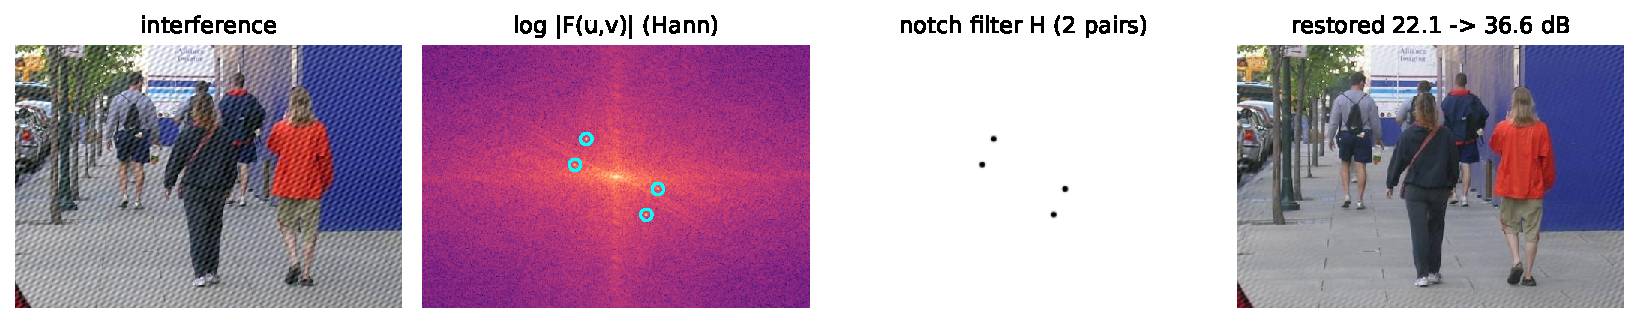
\includegraphics[width=0.85\textwidth]{exp2_notch_spectrum.pdf}
\caption{Automatic notch rejection. Left to right: interfered frame; its
Hann-windowed log-magnitude spectrum with the detected conjugate peak pairs
circled; the resulting Butterworth notch-reject filter $H(u,v)$; and the
restored frame.}
\label{fig:notch}
\end{figure*}

\subsubsection{The low-pass filter family and ringing}
On Gaussian noise the three transfer functions rank consistently
Gaussian $>$ Butterworth $>$ ideal at every cut-off: at $D_0{=}0.10$ they give
24.07, 23.59 and 22.79\,dB respectively. The ideal filter is worst despite
being the most aggressive, because its discontinuous transfer function has a
$\mathrm{sinc}$ impulse response that produces Gibbs ringing. Notably, at the tightest cut-off ($D_0{=}0.05$) the
ideal filter is \emph{worse than no filtering at all} in PSNR (20.33 versus
20.49\,dB): the ringing artefacts it introduces cost more than the noise it
removes. This is the classical textbook result \cite{gonzalez2018} reproduced
on real surveillance imagery, and it is why every low-pass in the deployed
pipeline is Gaussian.


\subsubsection{Uneven illumination}
Homomorphic filtering raises SSIM from 0.902 to \textbf{0.922} and PSNR from
16.83 to 18.17\,dB. CLAHE reaches a similar PSNR (18.03\,dB) but a \emph{lower}
SSIM (0.859), and global histogram equalisation is worse than doing nothing on
both (16.37\,dB, 0.849). The PSNR/SSIM divergence is instructive: CLAHE
improves average intensity error while damaging local structure, whereas the
homomorphic filter is the only method operating on the correct model---since
$f = i\cdot r$ is multiplicative, logarithms make it additive, so attenuating
low frequencies removes the illumination field rather than re-scaling the
histogram. A percentile stretch instead of the mean-restoring output mapping
lowers both metrics (14.84\,dB, 0.884).

\subsubsection{Frequency versus spatial implementation}
Filtering in the two domains is equivalent to within numerical precision: a
Gaussian applied as $H(u,v)$ and as a spatial kernel agree to 56.6--59.0\,dB
PSNR, which is round-off. The cost, however, is not equivalent. For
$\sigma{=}1$\,px the spatial convolution takes 0.29\,ms against 84.2\,ms for
the DFT route ($290\times$); even at $\sigma{=}8$\,px the spatial form remains
$24\times$ faster (3.6 versus 86.5\,ms), because the DFT cost is fixed by image
size while the spatial cost grows only with kernel support. The frequency
domain is therefore reserved in this system for operations with no compact
spatial equivalent---notch rejection and homomorphic filtering---rather than
used for ordinary smoothing.

\subsection{Task 3: Restoration and reconstruction}\label{sec:res-rest}
\subsubsection{Motion deblurring}
Table~\ref{tab:deblur} compares the three deconvolution filters on frames
blurred by a 15\,px horizontal motion PSF with additive noise.

\begin{table}[!t]
\caption{Deconvolution of a 15\,px motion blur ($\sigma{=}2$ noise), 30 images.}
\label{tab:deblur}
\centering
\scriptsize
\begin{tabular}{@{}lrrr@{}}
\toprule
\hdr{Method} & \hdr{PSNR} & \hdr{SSIM} & \hdr{ms} \\
\midrule
(degraded)                  & 22.49 & 0.653 & --- \\
inverse filter              & \textit{6.67} & \textit{0.027} & 50.4 \\
Wiener $K{=}0.001$          & 19.68 & 0.393 & 50.9 \\
Wiener $K{=}0.005$          & 24.27 & 0.586 & 50.4 \\
\textbf{Wiener $K{=}0.01$}  & \textbf{25.52} & 0.673 & 50.3 \\
Wiener $K{=}0.03$           & 25.20 & \textbf{0.751} & 50.1 \\
CLS $\gamma{=}0.02$         & 22.42 & 0.664 & 66.8 \\
Laplacian sharpen (no PSF)  & 19.02 & 0.390 & 3.5 \\
\bottomrule
\end{tabular}
\end{table}

The inverse filter is catastrophic: 6.67\,dB, i.e.\ 15.8\,dB \emph{worse} than
the blurred input it was meant to repair. This is the textbook failure made
concrete. Where $H(u,v)\to 0$ the quotient $G/H = F + N/H$ is dominated by
$N/H$, so the noise is amplified without bound. The Wiener filter differs only
by the additive term $K$ in the denominator, yet that term is the difference
between a 6.67\,dB result and a 25.52\,dB one. Its optimum is broad---$K$
between 0.005 and 0.03 all work---which matters in practice because $K$ is a
noise-to-signal ratio that must itself be estimated. Note also that PSNR and
SSIM disagree about the optimum ($K{=}0.01$ versus $K{=}0.03$): the larger $K$
suppresses more noise at the cost of residual blur, which SSIM rewards.


The PSF, however, must be known.
With the correct 15\,px length, Wiener yields 24.27\,dB; assuming 12\,px gives
22.16\,dB and assuming 18\,px gives 19.63\,dB. A $\pm20\,\%$ error therefore
costs 2.1--4.6\,dB, and at 21\,px (a 40\,\% over-estimate) the output at
17.86\,dB is \emph{worse than the blurred input}. Over-estimation is more
damaging than under-estimation because too long a PSF places spurious zeros
inside the signal band. Since no blind PSF estimator is implemented, the
deployed pipeline does not deconvolve, which is exactly why motion blur shows
the smallest detection gain in Table~\ref{tab:robust}.

\subsubsection{Low-light restoration and the ordering result}
One experiment justifies the pipeline's denoise-before-brighten ordering. On
night frames (8.60\,dB, SSIM 0.247 degraded), auto-gamma gives 16.76\,dB,
global histogram equalisation 17.57\,dB, CLAHE 12.38\,dB and gamma+CLAHE
15.92\,dB.

Crucially, denoising \emph{before} enhancement yields \textbf{18.37\,dB} and
SSIM \textbf{0.658}, while exactly the same two operations in the opposite
order yield 16.15\,dB and 0.526. The 2.2\,dB and 0.13\,SSIM difference comes
from nothing but ordering.
The reason is that the enhancement applies a gain of roughly $4\times$ to a
dark frame, and that gain multiplies the noise as surely as the signal; once
amplified and clipped, the noise cannot be removed as cleanly. This result is
what the gain-aware trigger in Fig.~\ref{fig:flowchart} implements: the
pipeline tests $\hat\sigma\cdot\gamma$ so that a dark, mildly noisy frame is
denoised \emph{before} it is brightened.

\subsubsection{Reconstruction of lost blocks}
Diffusion-based in-painting recovers packet loss almost completely. At 3\,\%
block loss, Telea in-painting raises PSNR from 21.60 to 35.00\,dB (+13.4\,dB)
in 5.5\,ms; at 1\,\% loss it reaches 40.38\,dB and at 8\,\% still 30.39\,dB.
Navier--Stokes in-painting is statistically indistinguishable (34.95\,dB at
3\,\%), so the cheaper Telea variant is the default. The naive alternative of
median filtering the damaged frame is not merely worse but actively harmful
(20.08\,dB at 3\,\% loss, below the 21.60\,dB degraded input), because it
smears the black blocks outward while also destroying undamaged detail. The
lesson generalises: reconstruction requires knowing \emph{which} pixels are
missing, which is precisely what the lost-block diagnostic provides at 100\,\%
detection (Table~\ref{tab:trigger}).

\subsection{Task 4: Segmentation}\label{sec:res-seg}
Table~\ref{tab:seg} compares both families inside the same ROIs, evaluated
against Penn-Fudan's pixel masks, first with oracle ground-truth boxes and then
with the YOLO boxes the deployed system actually produces.

\begin{table}[!t]
\caption{Segmentation inside person boxes (100 Penn-Fudan images). IoU/Dice
against pixel masks; time is per frame for all persons.}
\label{tab:seg}
\centering
\scriptsize
\begin{tabular}{@{}llrrrr@{}}
\toprule
\multirow{2}{*}{\hdr{Method}} & \multirow{2}{*}{\hdr{Family}} &
\multicolumn{2}{c}{\hdr{GT boxes}} & \multicolumn{2}{c}{\hdr{YOLO boxes}} \\
\cmidrule(lr){3-4}\cmidrule(lr){5-6}
 & & IoU & Dice & IoU & \hdr{ms} \\
\midrule
box (baseline)  & ---    & 0.497 & 0.658 & 0.473 & 0.1 \\
Canny + morph.  & edge   & 0.286 & 0.409 & 0.276 & 4.3 \\
Sobel + Otsu    & edge   & 0.201 & 0.306 & 0.179 & 4.3 \\
Otsu            & region & 0.426 & 0.579 & 0.404 & 6.2 \\
region growing  & region & 0.544 & 0.693 & 0.526 & 838 \\
\textbf{watershed} & region & \textbf{0.692} & \textbf{0.814} & \textbf{0.632} & \textbf{3.5} \\
GrabCut         & region & 0.642 & 0.766 & 0.588 & 401 \\
\bottomrule
\end{tabular}
\end{table}

Three conclusions follow. First, \emph{region-based methods dominate
edge-based ones} on cluttered streets (watershed 0.692 versus Canny 0.286):
pedestrian boundaries are often low-contrast, so an edge map is incomplete
where contrast is weak and over-complete where the background is textured, and
morphological closing cannot distinguish the two. Second, the best method is
also the cheapest competitive one---watershed is $115\times$ faster than
GrabCut \emph{and} more accurate, because a well-placed marker pair encodes the
same prior GrabCut must infer by iterating colour mixtures---so it is the
default in the \textsf{balanced} and \textsf{quality} profiles. Third, only
watershed and region growing beat the trivial ``fill the box'' baseline of
0.497. Replacing oracle with YOLO boxes costs a uniform 0.04--0.06 IoU, so
localisation error propagates but does not change the ranking.


\subsubsection{Does restoration help segmentation?}
Not consistently---a negative result worth stating. Under $\sigma{=}30$ noise,
watershed IoU falls from 0.641 (clean) to 0.541; \textsf{balanced} restoration
recovers only to 0.560 and \textsf{quality} (NLM) makes it \emph{worse} at
0.513. Canny degrades monotonically with denoising strength (0.302, 0.263,
0.240, 0.203). A strong denoiser removes the weak gradients both the edge
detector and the watershed transform rely on, and the noise it removed was not
what limited them. Restoration is justified by its effect on \emph{detection}
(Section~\ref{sec:res-rec}), not on segmentation.

\subsubsection{Motion segmentation on real CCTV}
On CAVIAR, background subtraction reaches $F_1$ 0.457--0.475 (MOG2) and
0.475--0.554 (running average) at 0.9--1.3\,ms per frame. MOG2 is more precise
(0.82--0.97) but less sensitive (recall 0.13--0.32), because its per-pixel
mixture absorbs a person who pauses into the background; the running average,
updated only where the pixel is currently background, retains such targets
longer. Both are an order of magnitude cheaper than a detector, and supply the
\textsf{fast} profile's segmentation.

\subsection{Task 5: Compression}\label{sec:res-comp}
\subsubsection{Rate--distortion}
Table~\ref{tab:rd} compares the production codec, our from-scratch DCT codec
and two wavelet codecs at matched bit rates, from measured byte counts.

\begin{table}[!t]
\caption{Quality at fixed rate (24 images), by linear interpolation of each
measured rate--distortion curve.}
\label{tab:rd}
\centering
\scriptsize
\begin{tabular}{@{}lrrrr@{}}
\toprule
\multirow{2}{*}{\hdr{Codec}} & \multicolumn{2}{c}{\hdr{0.5 bpp}} & \multicolumn{2}{c}{\hdr{1.0 bpp}} \\
\cmidrule(lr){2-3}\cmidrule(lr){4-5}
 & PSNR & SSIM & PSNR & SSIM \\
\midrule
JPEG (libjpeg)   & \textbf{27.01} & \textbf{0.801} & \textbf{30.69} & \textbf{0.902} \\
DCT codec (ours) & 25.80 & 0.761 & 29.07 & 0.863 \\
Wavelet bior4.4  & 25.19 & 0.698 & 29.02 & 0.824 \\
Wavelet Haar     & 24.42 & 0.663 & 27.96 & 0.795 \\
\bottomrule
\end{tabular}
\end{table}


Our DCT codec trails libjpeg by 1.6\,dB at 1\,bpp despite an identical
quantiser and IJG scaling. The difference is the entropy coder alone: libjpeg
uses optimised Huffman tables over run-length symbols, ours a generic zlib
stream over coefficient planes. Landing within 1.6\,dB of the production codec
validates the transform and quantisation stages. Among wavelets, CDF~9/7 beats
Haar by 0.8--1.1\,dB at equal rate; at 1\,bpp it matches our DCT codec in PSNR
but its SSIM is markedly lower (0.824 versus 0.863), reflecting diffuse ringing
rather than block edges.

\subsubsection{Task-aware fidelity: how far can we compress?}
PSNR is not the operational criterion; detection is. Re-running the detector on
JPEG-compressed frames gives pedestrian $F_1$ of 0.888 (raw, 24\,bpp), 0.878
($q{=}70$, 1.65\,bpp), \textbf{0.884} ($q{=}40$, 0.95\,bpp), 0.852
($q{=}20$), 0.778 ($q{=}10$) and 0.406 ($q{=}5$). Detection is therefore
\emph{unharmed} down to $q{=}40$---a $25\times$ reduction in data---and degrades
gracefully until it collapses below $q{=}10$. A surveillance network can
consequently transmit at roughly 1\,bpp without measurable analytic loss, which
is a far more useful operating rule than any fixed PSNR target.

\subsubsection{Region-of-interest coding}
The value of ROI coding depends entirely on how much of the frame the objects
occupy. On Penn-Fudan, whose pedestrians dominate the frame, ROI coding gains
only $0.5$\,dB on people (38.63 versus 38.14\,dB) while sacrificing 11\,dB of
background quality---a poor trade. On the wide CCTV view of
\texttt{vtest.avi}, where detected objects cover just \textbf{4.5\,\%} of the
pixels, the same scheme yields \textbf{35.06\,dB on objects against 28.04\,dB
for uniform JPEG at the same file size}, a gain of \textbf{7.0\,dB} for
2.9\,dB of background sacrifice.

This is the compression--fidelity trade-off resolved per region rather than per
frame, and it is only available because the recognition stage supplies the
object map---a direct, quantified module dependency
(Section~\ref{sec:interdep}). It also explains why the na\"ive experiment on a
close-up dataset would have concluded, wrongly, that ROI coding is not worth
implementing.

\subsection{Task 6: Object recognition}\label{sec:res-rec}
\subsubsection{Detector benchmark}
Table~\ref{tab:det} benchmarks the detectors on all 170 Penn-Fudan images
(423 labelled instances). YOLOv4-tiny at 416\,px is the best operating point on
every metric, and the classical HOG+SVM baseline is far behind
($F_1$ 0.576 versus 0.904).

\begin{table}[!t]
\caption{Detector benchmark, 170 Penn-Fudan images, 423 instances.}
\label{tab:det}
\centering
\scriptsize
\begin{tabular}{@{}lrrrrr@{}}
\toprule
\hdr{Detector} & \hdr{P} & \hdr{R} & \hdr{$F_1$} & \hdr{AP$_{50}$} & \hdr{ms} \\
\midrule
HOG + linear SVM          & 0.666 & 0.508 & 0.576 & 0.427 & 5.8 \\
YOLOv4-tiny @320          & 0.838 & 0.941 & 0.886 & 0.919 & 11.6 \\
\textbf{YOLOv4-tiny @416} & \textbf{0.855} & \textbf{0.960} & \textbf{0.904} & \textbf{0.926} & 16.1 \\
YOLOv4-tiny @608          & 0.724 & 0.917 & 0.809 & 0.807 & 27.8 \\
\bottomrule
\end{tabular}
\end{table}

The non-monotonic behaviour with input size is notable: enlarging the input
from 416 to 608\,px \emph{reduces} $F_1$ from 0.904 to 0.809. Recall barely
moves (0.960 to 0.917) while precision collapses (0.855 to 0.724) as false
positives more than double (69 to 148). At 608\,px the receptive field relative
to object size falls below the scales the COCO anchors were tuned for, so
background texture begins to fire the person class. For a resource-constrained
deployment the lesson is convenient: the most expensive setting is not merely
poor value, it is actively worse.

\subsubsection{Robustness and the value of restoration}
Table~\ref{tab:robust} is the central interdependence experiment: identical
detector, identical images, with and without the adaptive restoration stage.

\begin{table}[!t]
\caption{Pedestrian $F_1$ with and without adaptive restoration (30 images,
same detector throughout).}
\label{tab:robust}
\centering
\scriptsize
\begin{tabular}{@{}lrrr@{}}
\toprule
\hdr{Scenario} & \hdr{raw} & \hdr{+ balanced} & \hdr{+ quality} \\
\midrule
clean              & 0.900 & 0.917 & 0.906 \\
Gaussian $\sigma{=}15$ & 0.870 & 0.902 & 0.882 \\
Gaussian $\sigma{=}30$ & 0.803 & 0.828 & \textbf{0.867} \\
salt \& pepper 5\,\%   & 0.766 & 0.900 & \textbf{0.911} \\
salt \& pepper 20\,\%  & 0.624 & \textbf{0.917} & 0.910 \\
periodic               & 0.634 & 0.885 & \textbf{0.890} \\
motion blur            & 0.706 & \textbf{0.750} & 0.706 \\
low light              & 0.831 & \textbf{0.855} & 0.811 \\
uneven light           & 0.893 & \textbf{0.910} & 0.892 \\
block loss             & 0.911 & \textbf{0.917} & 0.899 \\
night compound         & 0.509 & 0.722 & \textbf{0.723} \\
\bottomrule
\end{tabular}
\end{table}

Restoration never harms the clean stream and recovers most of the loss on every
fault, with the largest gains exactly where the diagnostics fire hardest:
impulse noise ($+0.293$ $F_1$), periodic interference ($+0.256$) and compound
night ($+0.214$). Motion blur gains least ($+0.044$) because the pipeline does
not deconvolve---the PSF is unknown at run time. On the KITTI clip, vehicle
$F_1$ improves from 0.614 to 0.783 (Gaussian), 0.716 to 0.826 (impulse) and
0.567 to 0.809 (periodic), so the effect is not specific to pedestrians.

\subsubsection{Real CCTV: where the system actually fails}
Table~\ref{tab:caviar} evaluates the detectors on five CAVIAR sequences of
genuine surveillance footage. The spread is extreme and instructive.

\begin{table}[!t]
\caption{Detection on real CCTV (CAVIAR). $F_1$ tracks pedestrian pixel height,
not sequence difficulty in any other sense.}
\label{tab:caviar}
\centering
\scriptsize
\begin{tabular}{@{}lrrrr@{}}
\toprule
\multirow{2}{*}{\hdr{Sequence}} & \hdr{median} & \multicolumn{3}{c}{\hdr{$F_1$}} \\
\cmidrule(lr){3-5}
 & \hdr{height} & HOG & @416 & @608 \\
\midrule
EnterExitCrossingPaths1cor & 65\,px & 0.129 & \textbf{0.943} & 0.930 \\
OneLeaveShop1cor           & 61\,px & 0.038 & \textbf{0.820} & 0.798 \\
Meet\_Crowd                & 26\,px & 0.000 & 0.017 & 0.050 \\
Fight\_Chase               & 21\,px & 0.000 & 0.013 & 0.050 \\
Walk1                      & 18\,px & 0.000 & 0.062 & 0.097 \\
\bottomrule
\end{tabular}
\end{table}

$F_1$ correlates almost perfectly with median pedestrian height. The two
corridor views, where people occupy 61--65\,px, yield 0.943 and 0.820; the
three wide-angle lobby views, where the median person is 18--26\,px, collapse
to 0.013--0.097 for every detector. This is a scale limit, not a noise or
lighting limit: no restoration recovers a 20\,px person, because YOLOv4-tiny's
coarsest stride is comparable to the whole object. It is the most important
practical finding here, because it is invisible on Penn-Fudan---whose
pedestrians are hundreds of pixels tall---and would have been missed by
evaluating only on curated stills. The consequence is that camera placement
dominates algorithm choice: pedestrians must subtend roughly 40--50\,px, or
tiled per-tile inference must be added. HOG+SVM fails on all five sequences and
is not viable for real CCTV.

\subsubsection{Privacy versus accessibility}
Anonymising heads preserves the analytics: $F_1$ falls only from 0.900 to 0.877
(pixelation) or 0.872 (blurring), so counting and tracking still work on the
public stream, whereas pixelating whole bodies destroys them ($F_1$ 0.026).
Identity and detectability are separable only if the protected region is chosen
carefully. The keyed scrambler restores the original bit-exactly for a key
holder and yields an unrecoverable result under the wrong key.

\subsection{Real-time performance and resources}\label{sec:res-rt}
Table~\ref{tab:rt} reports the end-to-end throughput of all three profiles on
768$\times$576 video, on both a clean stream and a degraded night stream that
forces the restoration branch to execute.

\begin{table}[!t]
\caption{End-to-end performance, 768$\times$576, single process, full pipeline
including privacy and ROI coding.}
\label{tab:rt}
\centering
\scriptsize
\begin{tabular}{@{}llrrrr@{}}
\toprule
\hdr{Stream} & \hdr{Profile} & \hdr{FPS} & \hdr{ms} & \hdr{restore} & \hdr{detect} \\
\midrule
\multirow{3}{*}{clean}
 & fast     & \textbf{45.5} & 22.0 & 2.4 & 4.0 \\
 & balanced & 20.8 & 48.2 & 18.8 & 14.3 \\
 & quality  & 12.8 & 78.1 & 35.7 & 26.4 \\
\midrule
\multirow{3}{*}{night+noise}
 & fast     & \textbf{44.5} & 22.5 & 2.8 & 3.7 \\
 & balanced & 18.7 & 53.6 & 21.5 & 15.0 \\
 & quality  & 2.8 & 360.4 & 276.4 & 29.5 \\
\bottomrule
\end{tabular}
\end{table}

All three profiles exceed real time on a clean stream, and \textsf{fast} and
\textsf{balanced} remain real-time under degradation. \textsf{quality} is the
interesting case: 78\,ms on a clean frame but 360\,ms once the night stream
triggers non-local means, which alone costs 276\,ms. This is exactly what the
adaptive design intends---expensive operators are paid for only when the frame
warrants them---but it shows a worst-case latency budget must be sized for the
degraded case.

\begin{figure}[!t]
\centering
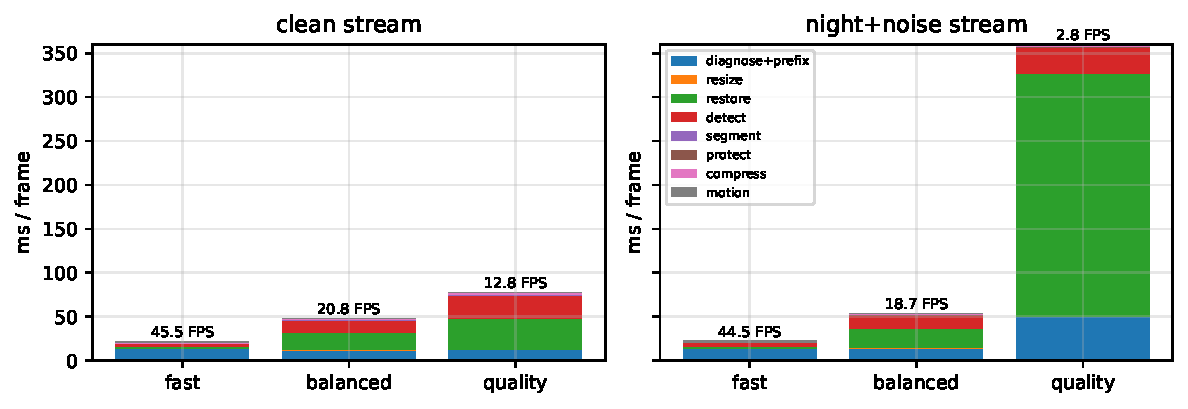
\includegraphics[width=0.92\columnwidth]{exp7_latency_breakdown.pdf}
\caption{Per-stage latency. On the clean stream in the \textsf{fast} profile,
blind diagnosis (13.5\,ms) is the dominant cost, not restoration or detection.}
\label{fig:latency}
\end{figure}

Fig.~\ref{fig:latency} exposes an unanticipated cost: in the \textsf{fast}
profile on a clean stream the diagnostic front end consumes 13.5 of the
22.0\,ms budget---more than detection and restoration combined. Diagnosis is
what allows every other stage to be skipped, so it is paid on every frame while
the stages it gates are not; amortising it over $N$ frames is the most valuable
remaining optimisation.

Detector input size is the principal speed control, spanning 7.6\,ms (224\,px,
132\,FPS) to 30.1\,ms (608\,px, 33\,FPS); with Table~\ref{tab:det}, 416\,px is
both the most accurate and a mid-cost setting, so the accuracy/speed trade-off
is unusually benign. Peak resident memory is 1292\,MB including the network and
the OpenCV runtime, fitting a Jetson- or Pi-5-class device.

%==============================================================================
\section{Module Interdependence}\label{sec:interdep}
%==============================================================================
\begin{figure*}[!t]
\centering
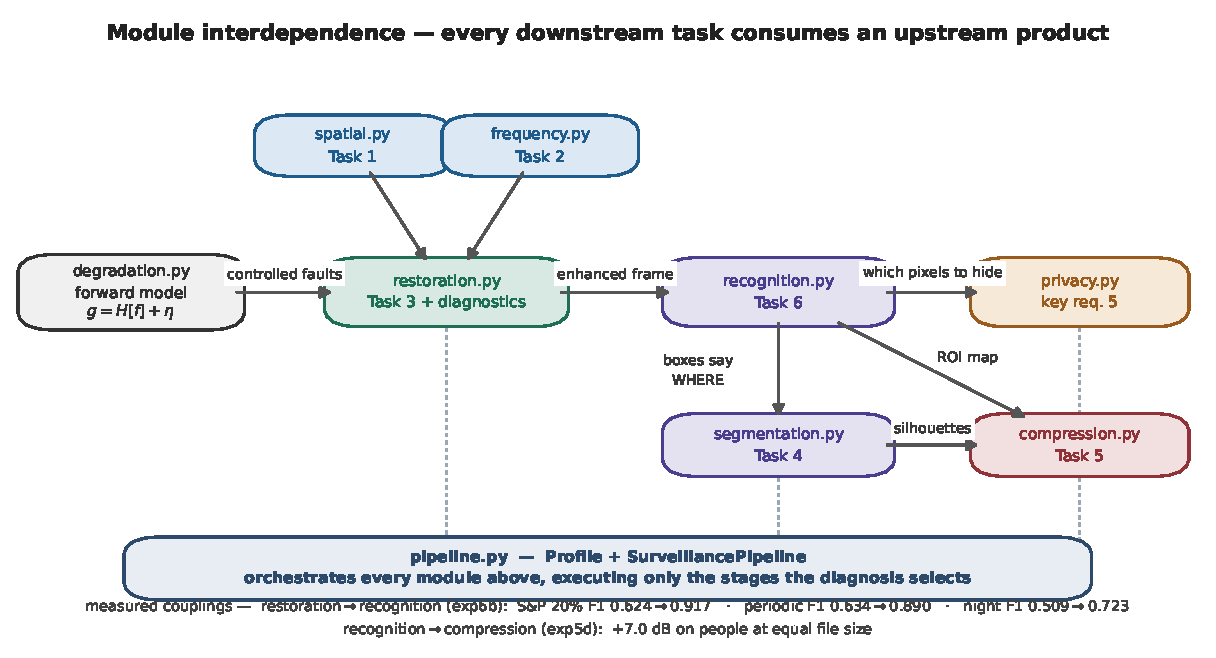
\includegraphics[width=0.82\textwidth]{fig_interdependence.pdf}
\caption{Module interdependence. Solid arrows are data dependencies; the
dashed ties indicate that \texttt{pipeline.py} orchestrates each module. The
captions carry the measured value of each coupling.}
\label{fig:interdep}
\end{figure*}

The interdependence of the modules deserves explicit analysis.
Fig.~\ref{fig:interdep} shows the dependency graph, and this project quantifies
each edge rather than asserting it.

\textit{Restoration $\rightarrow$ recognition} is the strongest coupling. The
same detector on the same scenes gains $+0.293$ $F_1$ under impulse noise,
$+0.256$ under periodic interference and $+0.214$ on compound night frames
(Table~\ref{tab:robust}). Restoration is not cosmetic; it is what makes the
detector usable on degraded input.

\textit{Recognition $\rightarrow$ segmentation} is a hard dependency: every
single-image segmenter runs inside a detector box, and substituting YOLO for
oracle boxes costs 0.04--0.06 IoU, so localisation error propagates but does
not dominate.

\textit{Recognition $\rightarrow$ compression} is worth the most bits:
detection-driven ROI coding yields $+7.0$\,dB on objects at equal file size
(Section~\ref{sec:res-comp}), because the codec can only protect regions the
detector identifies.

\textit{Recognition $\rightarrow$ privacy} determines what is hidden. Since the
head region derives from the detection box, a missed detection is also a
privacy failure---an availability requirement becomes a confidentiality one,
worth stating explicitly in a security review.

\textit{Restoration $\rightarrow$ segmentation} is the coupling that does
\emph{not} pay (Section~\ref{sec:res-seg}); segmentation consumes the restored
frame anyway because the detector needs it, so no un-restored path is kept.

%==============================================================================
\section{Discussion of the Key Trade-offs}\label{sec:tradeoffs}
%==============================================================================
We close by answering each of the five key requirements with a measurement.

\textit{Real-time versus quality.} The profiles span 45.5\,FPS
(\textsf{fast}) to 12.8\,FPS (\textsf{quality}) for a detection difference of
only 0.011 $F_1$ on clean frames but up to 0.064 on degraded ones. The correct
policy is therefore conditional---run \textsf{fast} until the diagnostics
report degradation, then escalate---and the diagnostics needed to implement it
already exist.

\textit{Resources versus performance.} Detector input size spans $4\times$ in
throughput and the accuracy optimum (416\,px) is not the most expensive
setting. Peak memory of 1292\,MB fits an edge device; no GPU is used.

\textit{Noise removal versus detail.} The adaptive median preserves detail a
fixed median destroys, and the gain-aware trigger avoids denoising frames that
do not need it. That over-filtering is real is clearest in segmentation: NLM
lowers watershed IoU from 0.560 to 0.513 against the cheaper bilateral filter.

\textit{Compression versus fidelity.} Pedestrian $F_1$ is unchanged to JPEG
$q{=}40$ (0.95\,bpp, $25\times$) and collapses below $q{=}10$. Fidelity the
analytics cannot perceive is worth discarding, and ROI coding discards it only
in the background.

\textit{Privacy versus accessibility.} Head anonymisation costs 0.023 $F_1$
while removing identity; whole-body anonymisation costs 0.874 and is unusable.
A keyed scrambler preserves lawful access and an HMAC tag makes tampering
detectable, serving three audiences---public, operator, investigator---from one
video store.

%==============================================================================
\section{Limitations and Future Work}\label{sec:limits}
%==============================================================================
\textit{Small objects dominate the error budget.} Detection fails below roughly
30\,px of pedestrian height regardless of restoration
(Table~\ref{tab:caviar}). Tiled inference, a higher-capacity detector or---most
cheaply---correct camera siting are the remedies. This is a property of the
detector and the geometry, not of the image-processing pipeline.

\textit{Uneven illumination is not blindly detectable}
(Section~\ref{sec:res-diag}), so homomorphic correction is exposed as a
per-camera installation setting rather than an automatic decision.

\textit{Deblurring assumes a known PSF.} Wiener restoration loses several dB
when the blur length is misestimated, so blind PSF estimation is the natural
next step; it is also why motion blur shows the smallest detection gain.

\textit{The noise estimator under-reads heavy noise} because of clipping, so
thresholds were calibrated against its measured output rather than nominal
$\sigma$.

\textit{The keyed scrambler is a teaching construction.} Block permutation with
a key-derived XOR keystream demonstrates reversible masking but is not an
authenticated cipher; a deployment should use AES-GCM with vaulted keys.

\textit{Synthetic degradation} is required because reference metrics need a
clean ground truth that real night footage cannot provide; the CAVIAR and
KITTI evaluations partially offset this with genuine footage.

%==============================================================================
\section{Conclusion}\label{sec:conclusion}
%==============================================================================
We presented an adaptive image-processing pipeline for smart-city surveillance
that diagnoses each frame blindly and executes only the restoration stages the
diagnosis justifies, under a profile capping the cost of each stage. All six
technical tasks are implemented, with the core operators written from first
principles and verified against reference libraries.

The measured outcomes: blind detection of five of six fault classes at 100\,\%
with at most 5\,\% false alarms; restoration lifting pedestrian $F_1$ from
0.624 to 0.917 under heavy impulse noise and 0.509 to 0.723 on compound night
frames; watershed segmentation at IoU 0.692 in 3.5\,ms, beating GrabCut on both
accuracy and cost; ROI coding worth $+7.0$\,dB on objects at equal file size;
and head anonymisation that removes identity for 0.023 $F_1$. The system runs
at 45.5\,FPS (\textsf{fast}) and 20.8\,FPS (\textsf{balanced}) on one CPU
within 1.3\,GB.

Two negative results are as informative as the positive ones. Denoising does
not improve segmentation, because strong denoisers remove the weak gradients it
depends on. And detection on genuine CCTV is governed by object scale rather
than image quality: below about 30\,px of pedestrian height every detector
fails regardless of restoration. The most valuable future work is therefore not
a better filter but blind PSF estimation, amortised diagnostics and tiled
inference for small objects.

\balance
% IEEE conference papers conventionally set the reference list smaller
\let\oldthebibliography\thebibliography
\renewcommand{\thebibliography}[1]{\oldthebibliography{#1}\scriptsize
  \setlength{\itemsep}{0pt plus 0.2pt}}
\bibliographystyle{IEEEtran}
\bibliography{refs}

\end{document}
